\documentclass[a4paper, 11pt]{article}
\usepackage{comment} % enables the use of multi-line comments (\ifx \fi) 
\usepackage{fullpage} % changes the margin
\usepackage{graphicx}
\usepackage{subfigure}
\usepackage{amsmath}
\usepackage{amsfonts}



\begin{document}
\noindent
\large\textbf{Final Exam} \hfill \textbf{Yen-Lin Chen} \\
\normalsize ECE 5412 \hfill yc2253@cornell.edu \\
Fall 2019 \hfill Due: 12/20/19 11 am\\

To make the notation consistent and clear, we (I) will use $x_k$ instead of $x[k]$ to denote the random variable $x$ at time $k$. 

\section*{Question 1}

\subsection*{1(a)}

In microelectronic circuits, people usually model the DC voltage as a small signal embedded in an AC background. The goal is then to uncover such small DC signal from the noisy measurements of the total DC+AC voltage. In this question, the small DC signal is modeled as a two-state Markov Chain, which can be the random switching of an electron between two energy orbitals in a device or an ion-channel in biology. 

On the other hand, in optical microscopy, some bio-fluorophores are triggered randomly according to the specific quantum yield. The emission and excitation wavelengths are sometimes so close that they cannot be separated by dichroic experimentally. Therefore, the measured signal is the linear combination of bright AC excitation laser beam and the weak DC emission plus noise. In such scenario, a more complex version of this model is applied. 



\subsection*{1(b)}
Since we know that the Markov Chain $s_k$ has two states: $+1$ and $-1$, it suffices to compute $p(s_k=1)$. We know the sensor model $y_k = s_k + A\sin(\omega k) + n_k$ so we have the following conditional probability on measurement. 
\begin{equation}
p(y_k|s_k) = \frac{1}{\sqrt{2\pi}}\exp\left[-\frac{1}{2}\left(y_k - s_k - A\sin(\omega k) \right)^2 \right]
\end{equation}
To derive the optimal filter equations, we start with the state at time $k$: $p(s_k=1)$ and use Chapman-Kolmogorov equation to obtain the prior at time $k+1$. 
\begin{equation}
p(s_{k+1}|y_{1:k}) = \sum_{s_k\in \{+1, -1\}} p(s_{k+1}|s_k)p(s_k)
\end{equation}
\begin{equation}
\begin{split}
p(s_{k+1}=1|y_{1:k}) & = p(s_{k+1}=1|s_k=1)p(s_k=1) + p(s_{k+1}=1|s_k=-1)p(s_k=-1) \\
 & = 0.8 p(s_k=1) + 0.2(1 - p(s_k=1)) \\ 
 & = 0.2 + 0.6 p(s_k=1)
\end{split}
\end{equation}
And $p(s_{k+1}=-1|y_{1:k}) = 1- p(s_{k+1}=1|y_{1:k}) = 0.8 - 0.6 p(s_k=1)$. Next, we apply Bayes rule to derive $p(s_{k+1}=1|y_{1:k+1})$. 
\begin{equation}
\begin{split}
 & p(s_{k+1}=1|y_{1:k+1}) = \frac{p(y_{k+1}|s_{k+1}=1)p(s_{k+1}=1|y_{1:k})}{\sum_{s_{k+1}\in \{+1, -1\}}p(y_{k+1}|s_{k+1})p(s_{k+1}|y_{1:k})}\\
 & = \frac{p(s_{k+1}=1|y_{1:k})\exp\left[-\frac{1}{2}\left(y_{k+1} - s_{k+1} - A\sin(\omega (k+1)) \right)^2 \right]}{\sum_{s_{k+1}\in \{+1, -1\}}p(s_{k+1}|y_{1:k})\exp\left[-\frac{1}{2}\left(y_{k+1} - s_{k+1} - A\sin(\omega (k+1)) \right)^2 \right]} \\ 
 & = p(s_{k+1}=1)
\end{split}
\end{equation}
Eq. (3-4) are the optimal filter equations. 



\subsection*{1(c)}

\begin{figure}
	\begin{center}
		\includegraphics[width=6.5in]{q1c.png}
		\caption{Question 1(c): (Top) The simulated sensor measurements from the model with $A = 2.5$, $\omega = 2\pi/60$ and the filtered estimate at every time point using the optimal filter equations. (Bottom) The difference between the measurements and the filtered estimate. The mean-square-error is $0.63$ in this case. }
	\end{center}
	\label{fig:q1c}
\end{figure}

We simulated 1000 sensor measurements and then implemented the optimal filter from part (b) and the traces are shown in the top of Fig. 1. The difference between the measurements and filtered estimates is shown in the bottom of Fig. 1 with the mean-square-error of $0.63$.  



\subsection*{1(d)}

We repeated the process of part (c) for 50 times and found the mean-square-error (MSE) of the filtered estimate to be $0.623$ with standard deviation of $0.036$. The low standard deviation suggests that the optimal filter is stable. We also found that the mean-square-error increases with smaller amplitude $A$ because the noise is on the same scale and the Markov Chain $s_k$ becomes difficult to uncover.  



\subsection*{1(e)}

For smoother, our goal is to derive the conditional probability $p(s_k=1|y_{1:N})$ where $k \leq N$. 
\begin{equation}
p(s_k=1|y_{1:N}) = \frac{p(s_k=1|y_{1:k})p(y_{k+1:N}|s_k=1)}{\sum_{i=1,-1}p(s_k=i|y_{1:k})p(y_{k+1:N}|s_k=i)}
\end{equation}
where the first term $p(s_k=1|y_{1:k})$ in the numerator is the forward filtered estimate of time $k$ given observations $y_{1:k}$, which is derived and computed in part (b) and (c). The second term $p(y_{k+1:N}|s_k=1)$ is the backward filter and we will derive in the following. 
\begin{equation}
\begin{split}
 & p(y_{k+1:N}|s_k=1) = p(y_{k+1}, y_{k+2:N}|s_k = 1)\\
 & = \sum_{j=1,-1} p(y_{k+2:N}|y_{k+1}, s_{k+1}=j, s_k=1)p(y_{k+1}, s_{k+1}=j|s_k=1)\\
 & = \sum_{j=1,-1} p(y_{k+2:N}|s_{k+1}=j)p(y_{k+1}|s_{k+1}=j)p(s_{k+1}=j|s_k=1)\\
 & = 0.2 + p(y_{k+2:N}|s_{k+1}=1)\left[0.8p(y_{k+1}|s_{k+1}=1)-0.2p(y_{k+1}|s_{k+1}=-1) \right]
\end{split}
\end{equation}
where $p(y_k|s_k)$ is given in Eq. (1). Therefore, we have a backward filtering recursion. Define $p_k = p(y_{k+1:N}|s_k=1)$ and $p_N = 1$. We have 
\begin{equation}
\begin{split}
p_k & = 0.2 + p_{k+1}\Bigg\{\frac{0.8}{\sqrt{2\pi}}\exp\left[-\frac{1}{2}\left(y_{k+1} - 1 - A\sin(\omega (k+1)) \right)^2 \right] \\
 & - \frac{0.2}{\sqrt{2\pi}}\exp\left[-\frac{1}{2}\left(y_{k+1} + 1 - A\sin(\omega (k+1)) \right)^2 \right]  \Bigg\}
\end{split}
\end{equation}
Therefore, the smoother equation in Eq. (5) is then 
\begin{equation}
p(s_k=1|y_{1:N}) = \frac{p(s_k=1)p_k}{p(s_k=1)p_k + (1-p(s_k=1))(1-p_k)}
\end{equation}
And the quantity $p(s_k=-1|y_{1:N})$ is simply $1-p(s_k=1|y_{1:N})$ for $k = 1,2,\dots, N$.

We implemented the smoother and filter on the same data to compare the MSE of both. The MSE's of the filter and smoother are found to be $0.6302$ and $0.5848$ respectively. The MSE of the smoother is smaller as expected. 



\subsection*{1(f)}

We repeated the process of part (e) for 50 times and found the mean-square-error (MSE) of the smoother to be $0.591$ with standard deviation of $0.038$. The MSE of the smoother is smaller than that of the optimal filter. 


\subsection*{1(g)}

Given the observation $Y_N = (y_1, y_2, \dots, y_N)$ and amplitude $A$, we can write down the complete likelihood $p(S_N, Y_N; A)$ as the following. 
\begin{equation}
p(S_N, Y_N; A) = \prod_{i=1}^N\frac{1}{\sqrt{2\pi}}\exp\left[-\frac{1}{2}(y_i - s_i - A\sin(\omega i))^2 \right]
\end{equation}
\begin{equation}
\log p(S_N, Y_N; A) = -\frac{N}{2}\log(2\pi) - \frac{1}{2}\sum_{i=1}^N\left[y_i-s_i-A\sin(\omega i) \right]^2
\end{equation}
where $\omega$ is known. We will derive the close-form expression of \textit{E-step} and parameter update in \textit{M-step} at the $I$\textsuperscript{th} iteration in the EM algorithm. 
\begin{enumerate}
\item \textit{E-Step}:

Our aim is now to evaluate the conditional expectation $Q(A, A^I) = E\left[\log p(S_N, Y_N; A) \middle| Y_N, A^I \right]$.
\begin{equation}
\begin{split}
Q(A, A^I) & = E\left[\log p(S_N, Y_N; A) \middle| Y_N, A^I \right]\\
 & = E\left[ -\frac{N}{2}\log(2\pi) \middle|Y_N, A^I \right] - E\left[ \frac{1}{2}\sum_{i=1}^Ny_i^2 \middle|Y_N, A^I \right] \\
 & - E\left[ \frac{1}{2}\sum_{i=1}^Ns_i^2 \middle|Y_N, A^I \right] - E\left[ \frac{1}{2}\sum_{i=1}^N A^2\sin^2(\omega i) \middle|Y_N, A^I \right] \\
 & + E\left[ \sum_{i=1}^N s_iy_i \middle|Y_N, A^I \right] + E\left[ \sum_{i=1}^NAy_i\sin(\omega i) \middle|Y_N, A^I \right] \\
 & - E\left[ \sum_{i=1}^N As_i\sin(\omega i) \middle|Y_N, A^I \right] \\
 & = \text{const} - \frac{1}{2}\sum_{i=1}^N A^2\sin^2(\omega i) + \sum_{i=1}^NAy_i\sin(\omega i)\\
 & - E\left[ \sum_{i=1}^N As_i\sin(\omega i) \middle|Y_N, A^I \right]\\ 
\end{split}
\end{equation}
\begin{equation}
Q(A, A^I) = \text{const} - \frac{1}{2}\sum_{i=1}^N A^2\sin^2(\omega i) + \sum_{i=1}^NAy_i\sin(\omega i) - A\sum_{i=1}^N E\left(s_i \middle| Y_N, A^I \right)\sin(\omega i)
\end{equation}
where the constant contains all the terms that do not involve $A$. The term $E\left(s_i \middle| Y_N, A^I \right)$ is the estimation of $s_i$ given $Y_N$, which can be evaluated using the smoother in part (e). 

\item \textit{M-Step}:

Now the goal is to find the update for parameter $A^{I+1}$ such that the conditional expectation $Q(A, A^I)$ is maximized. 
\begin{equation}
A^{I+1} = \text{arg}\max_{A} Q(A, A^I) \iff \frac{dQ}{dA}\Bigg|_{A^{I+1}}=0
\end{equation}
\begin{equation}
\frac{dQ}{dA} = 0 = -A^{I+1}\sum_{i=1}^N\sin^2(\omega i) + \sum_{i=1}^Ny_i\sin(\omega i) - \sum_{i=1}^N E\left(s_i\middle| Y_N, A^I \right)\sin(\omega i)
\end{equation}
\begin{equation}
A^{I+1} = \frac{\sum_{i=1}^N\left[ y_i - E\left(s_i\middle| Y_N, A^I \right)\right]\sin(\omega i) }{\sum_{i=1}^N\sin^2(\omega i)}
\end{equation}
\end{enumerate}

The \textit{E-Step} is to compute the state estimate $E\left(s_i\middle| Y_N, A^I \right)$ using the smoother while the \textit{M-Step} updates the parameter $A$ by Eq. (15). Note that although the full knowledge of the transition probability $P$ seems irrelevant in the EM algorithm, it appears heavily in computing the state estimate $E\left(s_i\middle| Y_N, A^I \right)$.


\subsection*{1(h)}

\begin{figure}
	\begin{center}
		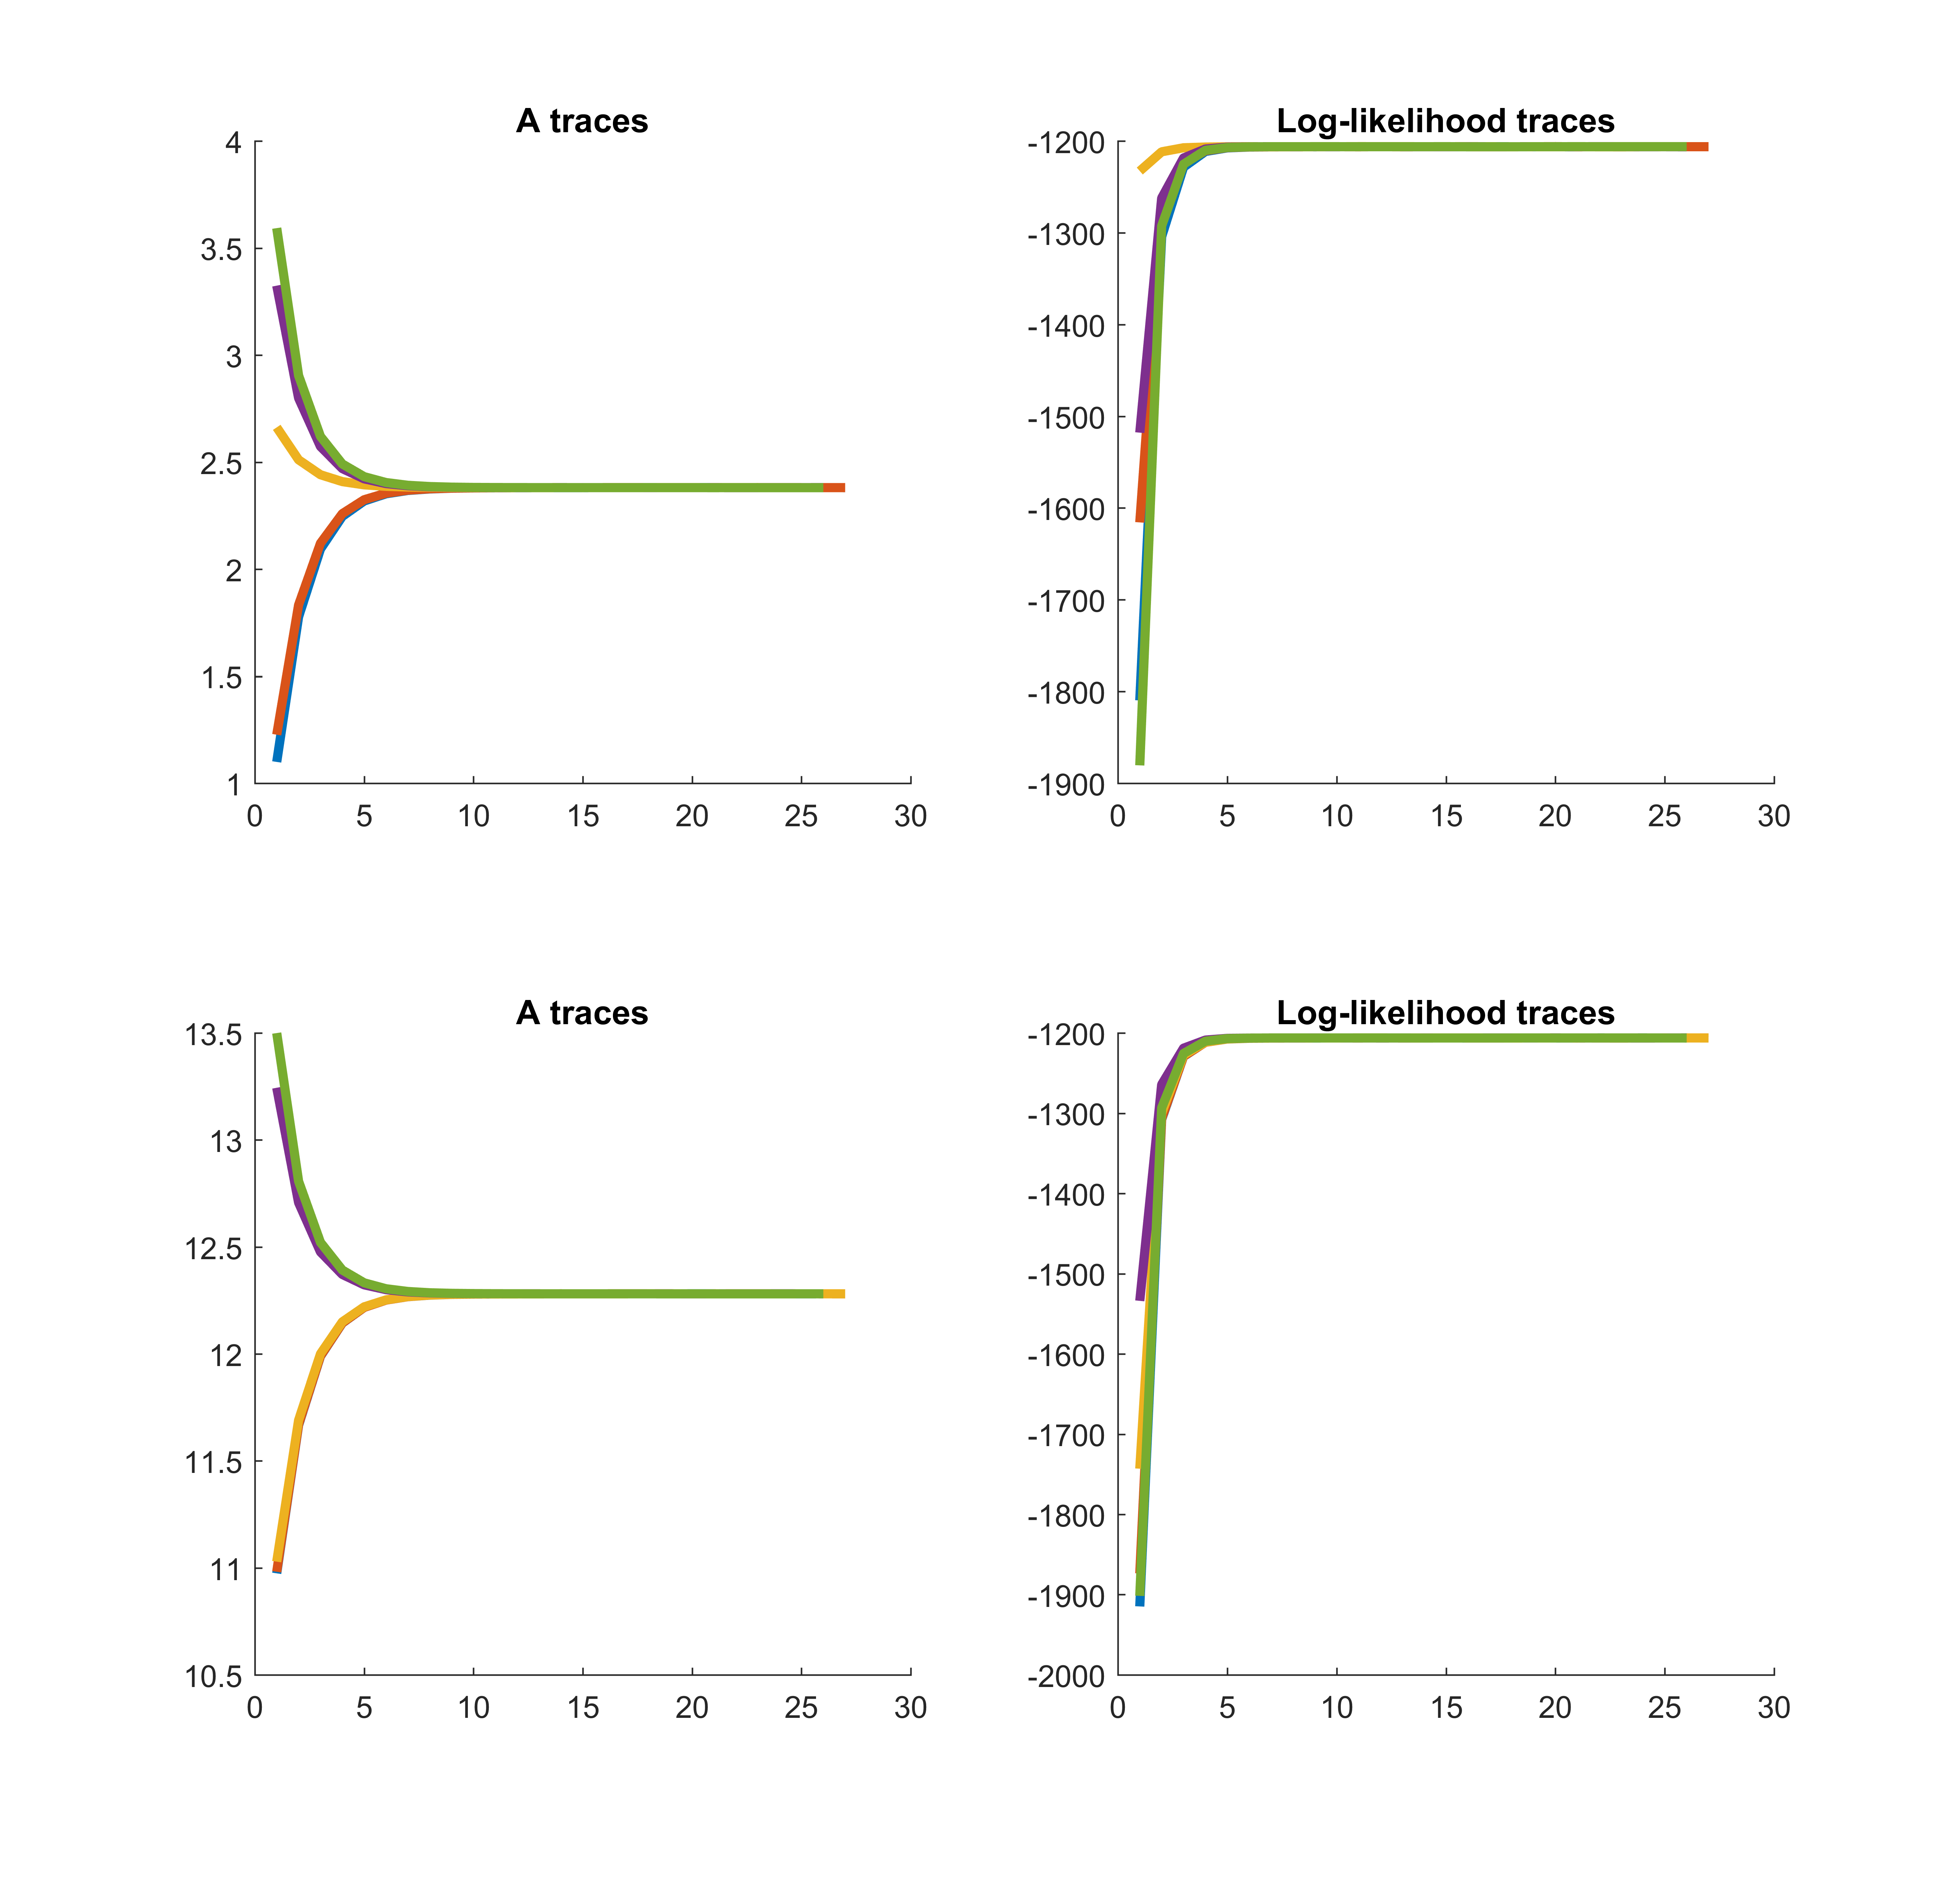
\includegraphics[width=7in]{q1h.png}
		\caption{Question 1(h): Traces of $A^I$ and log-likelihood of two experiments using 5 different starting values. }
	\end{center}
\end{figure}


We implemented the EM algorithm described above to obtain the maximum likelihood estimator of the amplitude $A$. The EM algorithm stops after the log-likelihood values stabilize. We use the variance of the latest $m$ iterations as the stopping criteria, where $m$ is chosen to be $10\%$ of the maximum iterations, $200$. The log-likelihood is as follows. 
\begin{equation}
\log p(Y_N|A) = -\frac{N}{2}\log(2\pi) - \frac{1}{2}\sum_{i=1}^N \left[y_i - E\left(s_i\middle| Y_N, A^I \right) - A\sin(\omega i) \right]^2
\end{equation}
We conducts two experiments with different $A$ values using 5 initial guesses. The traces of $A^I$ and log-likelihood versus iteration are shown in Fig. 2. The EM algorithm in this case converges fast (within 10 iterations) because it only involves estimation of one parameter. The log-likelihood is increasing with iterations as expected. The initialization of $A$ does not play an important role here since this is just the 1D case. In higher dimensions, EM algorithm might be stuck at local maximum of the rugged likelihood landscape. 



\section*{Question 2}
\subsection*{2(a)}


\begin{figure}
	\begin{center}
		\includegraphics[width=6.5in]{q2a.png}
		\caption{Question 2(a): The PDF and CDF from Metropolis-Hastings simulation and true function. }
	\end{center}
\end{figure}

We would like to simulate the following PDF using the random-walk Metropolis-Hastings (MH) algorithm. 
\begin{equation}
\pi(x) \propto \cos^2(x)\sin^2(2x)\psi(x) \quad \psi(x) = \mathcal{N}(0,1)
\end{equation}
The random-walk MH algorithm is implemented as the following steps. 
\begin{enumerate}
\item Given $x_k$, We use the symmetric Gaussian kernel to generate $x_{k+1}$, i.e. $x_{k+1}\sim\mathcal{N}(x_k, 1)$. 
\item Calculate the acceptance ratio $r$. 
\begin{equation}
r = \frac{\cos^2(x_{k+1})\sin^2(2x_{k+1})\psi(x_{k+1})}{\cos^2(x_k)\sin^2(2x_k)\psi(x_k)}
\end{equation}
\item Generate $u\sim [0,1]$ and accept $x_{k+1}$ if $u < r$ or go back to step 1. 
\end{enumerate}
The simulated PDF and CDF are shown in Fig. 3. 



\subsection*{2(b)}

The state model is given as follows. 
\begin{equation}
\begin{split}
x_{k+1} & = x_k + w_k, \quad w_k\sim\mathcal{N}(0,1)\\
y_k & = x_k + \left(v_k - \mu \right), \quad \mu = E\{v_k\}
\end{split}
\end{equation}
where the noise $v_k$ is given by part (a). Notice that the PDF in (a) is an even function so $\mu =  E\{v_k\} = 0$. We will apply the Kalman Filter (KF) to the system. 

Following the notation in class, since $A_k = C_k = Q_k = 1$ and $f_k = g_k = 0$, we have 
\begin{equation}
y_{k+1|k} = \hat{x}_{k+1|k} = \hat{x}_k
\end{equation}
Let the variance of $v_k$ be $R_{k}=\sigma^2$ and the KF equations are the following. 
\begin{equation}
\begin{split}
\hat{x}_{k+1} & = \hat{x}_k + \frac{1 + \Sigma_k}{1 + \sigma^2 + \Sigma_k}\left( y_{k+1} - \hat{x}_k \right) \\
\Sigma_{k+1} & = 1 + \Sigma_k - \frac{(1 + \Sigma_k)^2}{1 + \sigma^2 + \Sigma_k}
\end{split}
\end{equation}


\subsection*{2(c)}

\begin{figure}
	\begin{center}
		\includegraphics[width=6.5in]{q2c.png}
		\caption{Question 2(c): (Top) The traces of the simulated $y_k$ and KF estimate. (Bottom) The error percentage of the KF estimate. The error is at most $4\%$. The MSE is 0.23. }
	\end{center}
\end{figure}

We simulated $y_k$ where $k=1,2,\dots,1000$ and applied the Kalman Filter derived in part (b) to the $y$'s. Although the noise $v_k$ is not Gaussian, we approximate it with a Gaussian with zero mean and empirical variance $\text{Var}(v_k) = 0.71$. The traces of simulated measurements ($y_k$) and KF estimate are shown in the top panel of Fig. 4. The error percentage is shown in the bottom of Fig. 4, with maximum error percentage less than $4\%$. The MSE of the KF estimate is found to be $0.23$. 



\subsection*{2(d)}

The Kalman Filter estimate is the best linear unbiased estimator (BLUE) for non-Gaussian noise. In this case, if noise $v_k$ is iid Gaussian, the Kalman Filter is the optimal filter. However, $v_k$ is constructed from $\mathcal{N}(0,1)$ as a zero-mean noise with a smaller variance. The Kalman Filter approximates this iid non-Gaussian noise with $\mathcal{N}(0, \text{var}(v_k))$. There might be other non-linear optimal filters with better performance but the Kalman Filter is the best linear filter in this case. 



\subsection*{2(e)}

\begin{figure}
	\begin{center}
		\includegraphics[width=4.5in]{q2e.png}
		\caption{Question 2(e): The MSE of particle filter using both conditional and unconditional estimate with different number of particles $N$ compared to the MSE of Kalman Filter in (b). }
	\end{center}
\end{figure}

The bootstrap particle filter is implemented using the following steps. Suppose we can sample $N$ particles from the distribution $x^{(i)}_k\sim p(x_k|y_{1:k})$, our goal is to obtain the samples $x^{(i)}_{k+1}\sim p(x_{k+1}|y_{1:k+1})$ using the state space model defined in part (b).
\begin{enumerate}
\item Sample $x^{(i)} \sim \mathcal{N}(x^{(i)}_k, 1)$
\item Calculate the weights $w^{(i)} = p(y_{k+1}|x^{(i)})$, where 
\begin{equation}
p(y|x) = \pi(y-x) \propto \cos^2(y-x)\sin^2(2(y-x))\psi(y-x)
\end{equation} 
\item Sample $1:N$ according to the weights $w^{(i)}$, $I^{(i)}\sim w^{(i)}$
\item The new particles $x^{(i)}_{k+1} = x^{(I^{(i)})} \sim p(x_{k+1}|y_{1:k+1})$
\item The estimate of $x_{k+1}$ can be unconditional or conditional:
\begin{equation}
\begin{split}
\text{unconditional} & \quad\hat{x}_{k+1} = E(x_{k+1}|y_{1:k+1}) \approx \frac{1}{N}\sum_{i=1}^N x^{(i)}_{k+1}\\
\text{conditional} & \quad\hat{x}_{k+1} = E(x_{k+1}|y_{1:k+1}) \approx \frac{\sum_{i=1}^N w^{(i)}x^{(i)}_{k+1}}{\sum_{i=1}^N w^{(i)}}\\
\end{split}
\end{equation} 
\end{enumerate}

The bootstrap particle filter is implemented on the same data generated from the state space model with varying number of particles from $100$ to $3.3\times 10^5$. We show the conditional and unconditional MSE in Fig. 5 and the horizontal line is the MSE of the Kalman Filter. The difference between both estimate becomes subtle as number of particles increases. As the number of particles reaches above $3000$, the MSE is no longer improved. Compared to the performance of Kalman Filter, the bootstrap particle filter is slightly worse even with much more computational cost.


\section*{Notes on Codes}
The codes are written as MATLAB functions. The MATLAB scripts \textit{question1.m} and \textit{question2.m} contains sections that should reproduce all the plots and numbers here with sufficient comments. The rest of the files should be in the same directory. Comments are also included in the MATLAB functions.  


\end{document}
